% RESULTADOS-------------------------------------------------------------------

\chapter{RESULTADOS}
\label{chap:resultados}

%Cada capítulo deve conter uma pequena introdução (tipicamente, um ou dois parágrafos) que deve deixar claro o objetivo e o que será discutido no capítulo, bem como a organização do capítulo. 

Após a formulação e teste de cada item dos sistemas deu-se início a junção de todas as funcionalidades arquitetadas. O conteúdo deste capítulo visa apresentar os resultados obtidos neste trabalho em cada área de desenvolvimento.

Primeiramente como resultado da parte de \textit{hardware} podemos apresentar a formulação dos circuitos dos módulos \textbf{CCM} e \textbf{TCM} apresentados nas figuras abaixo. Os dois módulos foram montados em \textit{protoboard} buscando validar, em conjunto, todas funcionalidades as seções descritas na metodologia.


\begin{figure}[H]
	\centering
	\caption{Definição do \textit{layout} das telas criado no Figma.}
	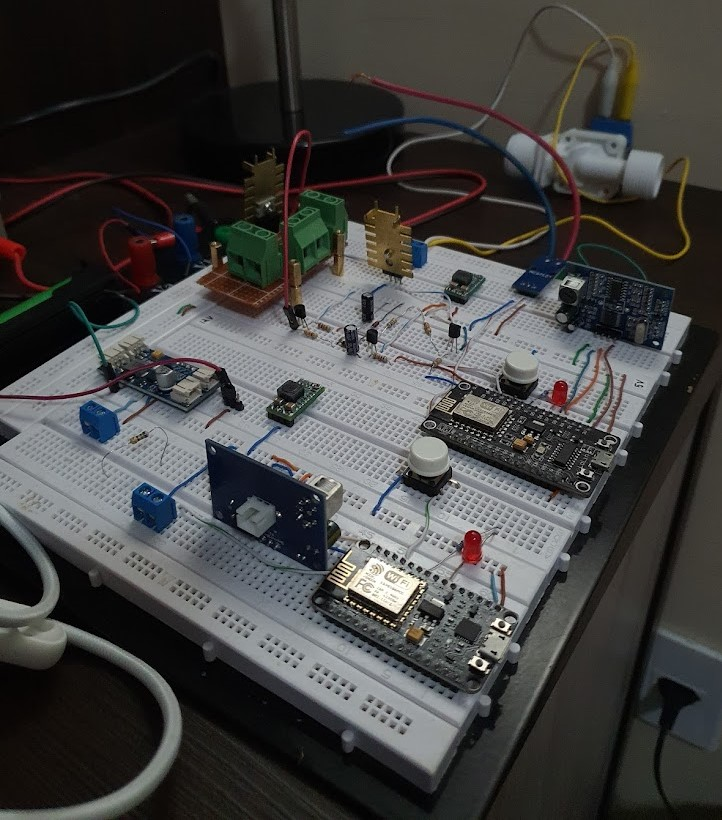
\includegraphics[width=0.6\textwidth]{figuras/esquema_protoboard.jpg}
	\fonte{Própria}
	\label{fig:figma_plan_desktop}
\end{figure}

Também foram desenvolvidos os esquemáticos dos dois módulos (\autoref{fig:kicad_ccm}), levando em consideração todas as ligações: circuitos de alimentação, sensoriamento e comunicação. Esse resultado garante futuras implementações de \textit{layout's 3D} e confecção das placas de circuito impresso.


\begin{figure}[H]
	\centering
	\caption{Definição do \textit{layout} das telas criado no Figma.}
	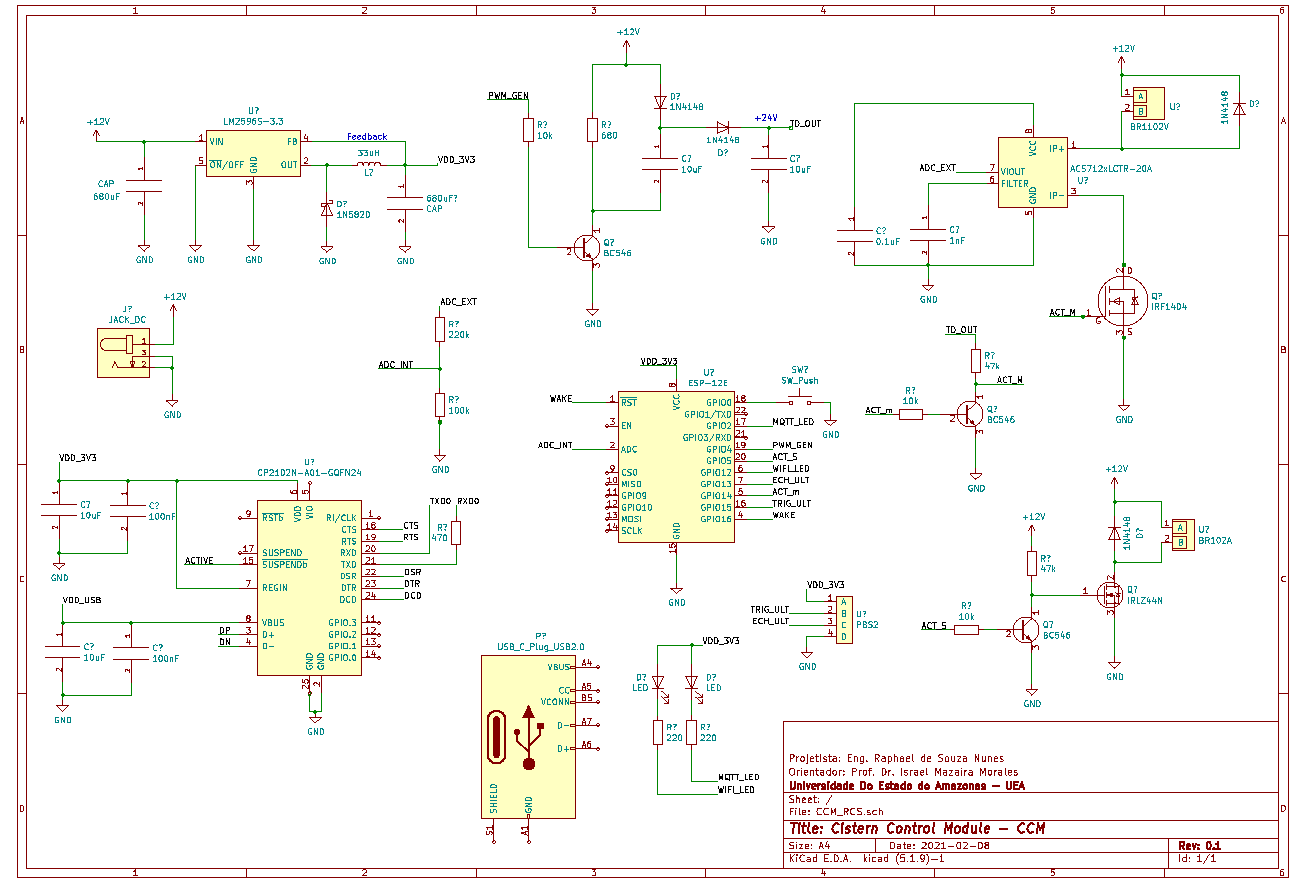
\includegraphics[width=1\textwidth]{figuras/kicad_ccm.png}
	\fonte{Própria}
	\label{fig:kicad_ccm}
\end{figure}



No quesito de \textit{firmware}, alcançou-se todas as funcionalidades propostas, gerando um código estável e escalável para projetos reais. Os códigos associados podem ser acessados no \textit{Github}.

\begin{figure}[H]
	\centering
	\caption{Definição do \textit{layout} das telas criado no Figma.}
	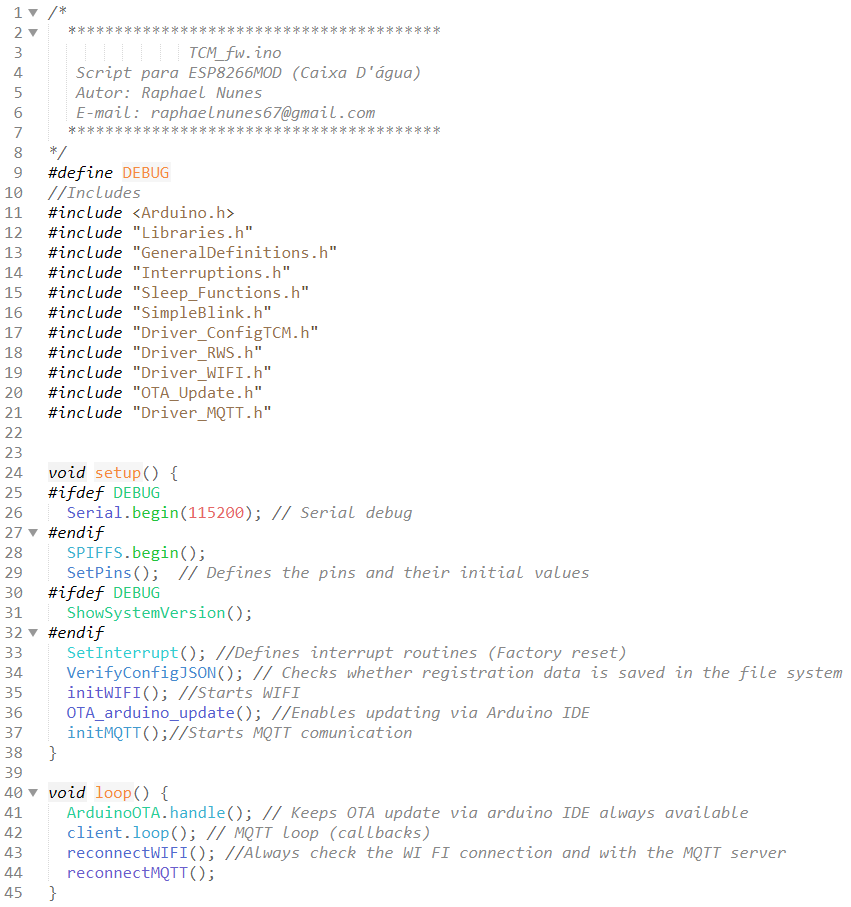
\includegraphics[width=1\textwidth]{figuras/tcm_main.png}
	\fonte{Própria}
	\label{fig:tcm_main}
\end{figure}


Por fim, também obtivemos como resultado a elaboração de telas utilizando as tecnologias propostas, atingindo o objetivo de relacionar o \textit{software} com as camadas de \textit{firmware} e \textit{hardware}. 